\documentclass[diploma]{softlab-thesis}


%%%
%%%  The document
%%%

\begin{document}

%%%  Title page

\frontmatter

\title{Μελέτη επίδρασης ανταγωνισμού για κοινούς πόρους σε περιβάλλον cloud}
\author{Κωνσταντίνος Παπαδημητρίου}
\date{Φεβρουάριος 2017}
\datedefense{17}{1}{2017}

\supervisor{Γεώργιος Γκούμας}
\supervisorpos{Αν. Καθηγητής Ε.Μ.Π.}

\committeeone{Γεώργιος Γκούμας}
\committeeonepos{Αν. Καθηγητής Ε.Μ.Π.}
\committeetwo{Νικόλαος Παπασπύρου}
\committeetwopos{Αν. Καθηγητής Ε.Μ.Π.}
\committeethree{Νεκτάριος Κοζύρης}
\committeethreepos{Καθηγητής Ε.Μ.Π.}

\TRnumber{CSD-SW-TR-42-14}  % number-year, ask nickie for the number
\department{Τομέας Τεχνολογίας Πληροφορικής και Υπολογιστών}

\maketitle


%%%  Abstract, in Greek

\begin{abstractgr}%
Σκοπός της παρούσης εργασίας είναι η ανάλυση βασικών αλγορίθμων χρονοδρομολόγησης σε περιβάλλον cloud computing, δηλαδή
θα δούμε πόσο περίπου βγαίνει..

Σε λίγο θα ξενερώσω περισσότερο..
\begin{keywordsgr}
Γλώσσες προγραμματισμού, Προγραμματισμός με αποδείξεις, Ασφαλείς γλώσσες
προγραμματισμού, Πιστοποιημένος κώδικας.
\end{keywordsgr}
\end{abstractgr}


%%%  Abstract, in English

\begin{abstracten}%
  The purpose of this diploma dissertation is on one hand the design
  of a simple high-level language that supports programming with
  proofs, and on the other hand the implementation of a compiler for
  this language. This compiler will produce code for an
  intermediate-level language suitable for creating certified
  binaries.

  The need for reliable and certifiably secure code is even more
  pressing today than it was in the past. In many cases, security and
  software compatibility issues put in danger the operation of large
  systems, with substantial financial consequences. The lack of a
  formal way of specifying and proving the correctness of programs that
  characterizes current programming languages is one of the main reasons
  why these issues exist. In order to address this problem, a number of
  frameworks with support for certified binaries have recently been
  proposed. These frameworks offer the possibility of specifying and
  providing a formal proof of the correctness of programs. Such a proof
  can easily be checked for validity before running the program.

  The frameworks that have been proposed are intermediate-level in
  nature, thus the process of programming in these is rather cumbersome.
  The high-level languages that accompany some of these frameworks,
  while very expressive, are hard to use. A simpler high-level language,
  like the one proposed in this dissertation, would enable further use
  of this programming idiom.

  In the language we propose, the programmer specifies the partial
  correctness of a program by annotating function definitions with pre-
  and post-conditions that must hold for their parameters and results.
  The programmer also provides a set of theorems, based on which proofs
  of the proper implementation and use of the functions are constructed.
  An implementation in OCaml of a compiler from this language to the
  NFLINT certified binaries framework was also completed as part of this
  dissertation.

  We managed to keep the language close to the feel of the current
  widespread functional languages, and also to fully separate the
  programming stage from the correctness-proving stage. Thus an average
  programmer can program in a familiar way in our language, and later an
  expert on formal logic can prove the semi-correctness of a program.
  As evidence of the practicality of our design, we provide a number of
  examples in our language with full semi-correctness proofs.
\begin{keywordsen}
Programming languages, Programming with proofs, Secure programming
languages, Certified code.
\end{keywordsen}
\end{abstracten}


%%%  Acknowledgements

\begin{acknowledgementsgr}
Ευχαριστώ θερμά τον επιβλέποντα καθηγητή αυτής της διατριβής,
κ.~Γιάννη Παπαδάκη, για τη συνεχή καθοδήγηση και εμπιστοσύνη
του. Ευχαριστώ επίσης τα μέλη της συμβουλευτικής επιτροπής,
κ.κ.~Νίκο Παπαδόπουλο και Γιώργο Νικολάου για την πρόθυμη και
πάντα αποτελεσματική βοήθειά τους, τις πολύτιμες συμβουλές και
τις χρήσιμες συζητήσεις που είχαμε.  Θέλω να ευχαριστήσω ακόμα
τον συμφοιτητή και φίλο Πέτρο Πετρόπουλο, ο οποίος με βοήθησε σε
διάφορα στάδια αυτής της εργασίας.  Θα ήθελα τέλος να ευχαριστήσω
την οικογένειά μου και κυρίως τους γονείς μου, οι οποίοι με
υποστήριξαν και έκαναν δυνατή την απερίσπαστη ενασχόλησή μου τόσο
με την εκπόνηση της διπλωματικής μου, όσο και συνολικά με τις
σπουδές μου.
\end{acknowledgementsgr}


%%%  Various tables

\tableofcontents
%\listoftables
%\listoffigures


%%%  Main part of the book

\mainmatter

\chapter{Εισαγωγή}
\section{Αρχές πολυπύρηνων αρχιτεκτονικών}
Τα τελευταία χρόνια η σχεδίαση και οι αρχές των υπολογιστικών συστημάτων έχουν
αλλάξει ραγδαία. Αρχικά ένας επεξεργαστής αποτελούνταν από ένα μόλις πυρήνα ο
οποίος  αναλάμβανε να εκτελέσει όλη την εργασία. Αυτό φυσικά καυτστερεί
ιδιαίτερα τις διάφορες εφαρμογές και δεν εκμεταλεύεται τις δυνατότητες
παραλληλισμού είτε εντός της εφαρμογής είτε μεαταξύ δύο η περισσότερων
εφαρμογών. Έτσι η πρόοδος της τεχνολογίας και οι απαιτήσεις για μεγάλη
υπολογιστική δύναμη έφεραν τις πολυπύρηνες αρχιτεκτονικών, στις οποίες ο φόρτος
εργασίας διαμοιράζεται σε περισσότερους πυρήνες, βελτιώνοντας θεαματικά την
απόδοση ενός συστήματος.

Η τεχνολογία των πολυπύρηνων αρχιτεκτονικών ήταν γνωστή και χρησιμοποιούταν από
τις προηγούμενες δεκαετίες σε συστήματα μεγάλης κλίμακας όπως υπερυπολογιστές
και κέντρα δεδομένων (data centers). Είναι τα τελευταία χρόνια όμως που έχει
γνωρίσει μεγάλη άνθηση. Η μεγάλη ζήτηση σε αποδοτικότερα συστήματα έφερε την
τεχνολογία σε υπολογιστές και συστήματα γενικού σκοπού όπως laptop και κινητά
τηλέφωνα.
Ωστόσο, τα συστήματα αυτά συναντάνε νέα προβλήματα (ΠΡΕΠΕΙ ΝΑ ΒΑΛΩ ΤΑ ΠΡΟΒΛΗΜΑΤΑ
ΤΩΝ ΜΟΝΟΠΥΡΗΝΩΝ ΑΡΧΙΤΕΚΤΟΝΙΚΩΝ) τα οποία περιορίζουν την βελτίωση της
απόδοσης/υπολογιστικής ισχύος. Οι πυρήνες μοιράζονται κοινούς πόρους για τη
χρήση/χρησιμοποίηση των οποίων ανταγωνίζονται. Αυτό έχει ως αποτέλεσμα τον
περιορισμό της συνολικής επίδοσης (throughput). Είναι δουλειά λοιπόν του
λειτουργικού συστήματος να μοιράσει με τέτοιο τρόπο τους πόρους στις διάφορες
εφαρμογές ώστε να ελαχιστοποιείσει αυτόν τον ανταγωνισμό.
\section{Λειτουργικά Συστήματα}
Με τον όρο λειτουργικό σύστημα (Operating System - OS) εννοούμε το πρόγραμμα το
οποίο αναλαμβάνει να διαμοιράσει τους πόρους του συστήματος στις διάφορες
διεργασίες. Βασικός ρόλος λοιπόν του ΛΣ είναι να δίνει χρόνο για εκτέλεση στις
εφαρμογές και να διαμοιράζει την κύρια μνήμη όπως και τους λοιπούς πόρους.
Επίσης αναλαμβάνει να διατειρεί τα διάφορα συστήματα αρχείων και να παρέχει στις
διεργασίες ό,τι μπορεί να χρειαστούν.

Για την επίλυση του προαναφερθήσαντος προβλήματος το ΛΣ πρέπει να λαβμάνει υπ'
όψη τις απαιτήσεις των διεργασιών και να παίρνει διάφορες αποφάσεις αναφορικά με
τον διαμοιρασμό/την παροχή των πόρων. Βασικό συστατικό ενός ΛΣ αποτελεί ο
χρονοδρομολογητής (scheduler). Ο χρονοδρομολογητής παίρνει αποφάσεις βασισμένες
σε μια συγκεκριμένη πολιτική και αφορούν τη χρήση του επεξεργαστή από τις
διεργασίες με στόχο τη βέλτιστη απόδοση του συστήματος. Η απόδοση από τη μεριά
της μπορεί να μεταφράζεται είτε σε καλή αποκρισιμότητα - χαρακτηριστικό
απαραίτητο σε συστήματα γενικού σκοπού, είτε σε υψηλό throughput, δηλαδή
επεξεργασία μεγάλου όγκου δεδομένων ανα μονάδα χρόνου - απαραίτητο σε συστήματα
μεγάλης κλίμακας, όπως servers και υπερυπολογιστές.

Έχουν προταθεί και υλοποιηθεί λοιπόν πολλές πολιτικές/αλγόριθμοι που αποφασίζουν
την σειρά και με την οποία οι διάφορες διεργασίες θα καταλάβουν/χρησιμοποιήσουν
την κεντρική μονάδα επεξεργασίας (ΠΡΕΠΕΙ ΝΑ ΓΕΜΙΣΟΥΜΕ ΚΑΙ ΣΕΛΙΔΕΣ!!!). Για
συστήματα με μόνο μία μονάδα επεξεργασίας, το πρόβλημα ανάγεται στον διαμοιρασμό
του χρόνου στις διεργασίες που χρειάζονται τον επεξεργαστή και μετά από έρευνες
ετών οι πολιτικές που είχαν προταθεί βελτιστοποιήθηκαν. Με την πρόοδο
ωστόσο της τεχνολογίας και την είσοδο στις πολυπύρηνες αρχιτεκτονικές η
πολυπλοκότητα του προβλήματος αυξήθηκε καθώς πλέον δεν πρέπει να διαμοιραστεί
μόνο ο χρόνος αλλά να αποφασιστεί και ποιος πυρήνας θα διατεθεί στην εκάστοτε
διεργασία. Οι υπάρχουσες υλοποιήσεις που χρησιμοποιούνται στα σημερινά λειτουργικά
συστήματα δεν λαμβάνουν υπ' όψιν την πολυπλοκότητα του συστήματος και
χειρίζονται τους πυρήνες ως ξεχωριστές οντότητες. Αυτή η λογική ενώ είναι αρκετά
απλή και εύκολα υλοποιήσιμη, έχει συχνά ως συνέπεια την ταυτόχρονη εκτέλεση
διεργασιών που χρησιμοποιούν κοινούς πόρους, με αποτέλεσμα την αύξηση του
ανταγωνισμού και τον περιορισμό της απόδοσης του συστήματος.

..
\section{Υπολογιστικό Νέφος (Cloud Computing)}
Τα τελευταία χρόνια προωθείται με νέα τάση, όπου ο χρήστης δεν χρησιμοποιεί
μηχανήματα της κατοχής του για υπολογισμούς ή αποθήκευση δεδομένων, αλλά προτιμά
οργανισμούς ή εταιρείες που είναι σε θέση να παρέχουν τις εν λόγω υπηρεσίες.
Υπολογιστικό νέφος (Cloud Computing) είναι ένας τύπος υπηρεσίας, βασισμένης στο
διαδίκτυο, όπου ένας χρήστης μπορεί να χρησιμοποιήσει απομακρυσμένα συστήματα
για προσωπική χρήση. Έτσι μία οντότητα που μπορεί να είναι είτε απλός χρήστης είτε
οργανισμός ή εταιρεία έχει τη δυνατότητα να μισθώσει μηχανήματα που δεν έχει
στην κατοχή της και να γλιτώσει τουλάχιστον αρχικά το κόστος αγοράς και
εγκατάστης δικού της κέντρου δεδομένων. 

\subsection{Μοντέλα Νεφών}
Τα βασικά μοντέλα υπηρεσιών που παρέχει ένα νέφος χωρίζονται σε αφαιρετικά
επίπεδα και είναι τα εξής:

\begin{wrapfigure}{r}{0.38\textwidth}
	\centering
	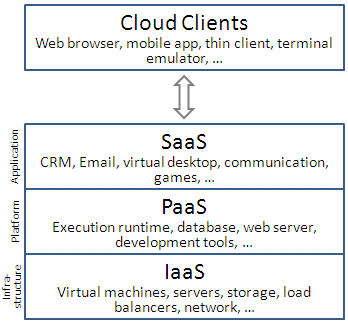
\includegraphics[scale=0.5]{cloud}
\end{wrapfigure}

\textbf{Λογισμικό ως Υπηρεσία - Software as a Service (SaaS)}. Σε αυτόν τον
τύπο, ο τελικός χρήστης / πελάτης έχει την δυνατότητα να χρησιμοποιήσει τις
εφαρμογές που του δίνει ο πάροχος και τρέχουν στο νέφος. Οι εφαρμογές γίνονται
προσβάσιμες από τον χρήστη μέσω κάποιας διεπαφής (πχ web browser, command-line
interface κλπ). Ο πελάτης δεν έχει την δυνατότητα να τροποποιήσει τις υποδομές
του νέφους (όπως το δίκτυο, τους αποθηκευτικούς χώρους ή το λειτουργικό σύστημα)
παρα μόνο την εφαρμογή που του παρέχεται, τις ρυθμίσεις της και το περιβάλλον
της. Τυπικά παραδείγματα SaaS είναι εφαρμογές email, εικονικές επιφάνειες
εργασίας και online παιχνίδια.

\textbf{Πλατφορμα ως Υπηρεσία - Platform as a Service (PaaS)}. %to be filled
To be filed

\textbf{Υποδομή ως Υπηρεσία - Infrastructure as a Service (IaaS)}. Εδώ ο
χρήστης έχει τη δυνατότητα να δημιουργήσει και να ελέγξει το σύστημα που θα
χρησιμοποιήσει, δηλαδή να επιλέξει χαρακτηριστικά όπως το λειτουργικό σύστημα η
τοπολογία του δικτύου κ.ο.κ αλλά και πάλι δεν μπορεί να τροποποιήσει το
υποκείμενο σύστημα πάνω στο οποίο τρέχουν οι υπηρεσίες εκτός ίσως από
περιορισμένο αριθμό ρυθμίσεων, όπως το τοίχος προστασίας του host (firewall).
Τυπικό παράδειγμα αυτού του τύπου των υπηρεσιών είναι η εικονικές μηχανές και ο
εικονικός/απομακρυσμένος (?) αποθηκευτικός χώρος. Στην περίπτωση των εικονικών
μηχανών, ο χρήστης δημιουργεί εικονικά μηχανήματα, τα οποία υλοποιούνται με
κάποιον hypervisor στο απομακρυσμένο σύστημα και ο πελάτης έχει πλήρη πρόσβαση
σε αυτά. Ο τρόπος με τον οποίο τα εικονικά μηχανήματα τοποθετούνται στους
επεξεργαστές του host είναι το αντικείμενο μελέτης της παρούσας εργασίας.

\subsection{Πλεονεκτήματα}
Ίσως το σημαντικότερο πλεονέκτημα του νέφους είναι η σημαντική εξοικονόμηση κόστους
και ενέργειας. Ο χρήστης έχει τις υπηρεσίες που χρειάζεται, όταν τις χρειάζεται
χωρίς να απασχολείται για το που και πως θα βρει την υπολογιστική ισχύ που
απαιτείται και χωρίς να πρέπει να αγοράσει υπερκοστολογιμένα μηχανήματα.
Αντίστοιχα μία εταιρεία μπορεί να είναι πλήρως λειτουργική με σχεδόν μηδενικό
κόστος.

Επίσης πολύ σημαντική είναι η ευκολία και η διαθεσιμότητα των υπηρεσιών από
οποιοδήποτε σημείο βρίσκεται ο τελικός χρήστης. Με απλές μεθόδους (login) ο
χρήστης έχει πλήρη πρόσβαση στις εικονικές μηχανές του ή στα απομακρυσμένα
δεδομένα που έχει αποθηκεύσει. Άλλωστε ο πάροχος αναλαμβάνει την προστασία των
δεδομένων και την ασφαλή επαναφορά τους μετά από απώλεια, κρατώντας πολλά αντίγραφα
στο νέφος. Σε περίπτωση κάποιας αναπόφευκτης αστοχίας, ο τελικός χρήστης δεν
θα χρειαστεί να διαθέσει ούτε χρόνο ούτε ανθρώπινο δυναμικό για την επισκευή
βλαβών.

Η χρήση του νέφους παρέχει μεγάλη ευελιξία. Το κόστος (είτε χρηματικό, είτε
ενεργειακό, είτε εξοπλιστικό) είναι άμεσα συνδεδεμένο με τις !current! ανάγκες
του χρήστη. Έτσι αν μία εταιρεία χρειαστεί παραπάνω πόρους για συγκεκριμένο /
προκαθορισμένο χρονικό διάστημα το μόνο που έχει να κάνει είναι να τους
νοικιάσει από κάποιο πάροχο αντί να υποστεί το πλήρες αντίτιμο για αυτούς (ή
κάτι τέτοιο τεσπα)

\subsection{Μειονεκτήματα}
Όπως όλες οι νέες τεχνολογίες, εκτός από θετικά υπάρχουν και κάποια αρνητικά. Με
τη χρήση του νέφους, υπάρχει ο -έστω και αμυδρός- κίνδυνος τεχνικής βλάβης για
την οποία δεν ευθύνεται ο χρήστης. Τυπικά οι πόροι είναι μόνιμα διαθέσιμοι
από διαφορετικές τοποθεσίες, ωστόσο η πρόσβαση σε αυτούς γίνεται μέσω
διαδικτύου που ακόμα και σήμερα δεν θεωρείται πάντα δεδομένη.

Επίσης σημαντική είναι η ασφάλεια των δεδομένων. Μία εταιρεία εμπιστεύεται μέρος
των δεδομένων της σε τρίτους, χωρίς να μπορεί να διασφαλίσει πως αυτά δεν θα
υποκλαπούν. Άλλωστε η κρυπτογράφησή τους μπορεί να μειώσει πολύ την απόδοση του
εγχειρήματος. Παρόμοια, η ιδιοτικότητα ευαίσθητων δεδομένων δεν μπορεί να
θεωρείται δεδομένη.

\section{Εικονικές Μηχανές (VM)}
Η έννοια των εικονικών μηχανών υπάρχει από την δεκαετία του 1960 αλλά είναι τα
τελευταία 10 χρόνια που έχει επανέλθει στο προσκήνιο, κυρίως επειδή η υψηλή
υπολογιστική ισχύς των σύγχρονων συστημάτων προσφέρει τη δυνατότητα υλοποίησής
τους. Με τον όρο εικονοποίηση, εννοούμε τη δημιουργία εικονικών αντικειμένων
(αντί πραγματικών) όπως εικονικές πλατφόρμες, δίκτυα, συσκευές αποθήκευσης κλπ.
Τα πλεονεκτήματα από τη χρήση εικονικών μηχανών είναι πολλά. Κάποια είναι
περισσότερο  προφανή, όπως η εκτέλεση εφαρμογών που δεν έχουν σχεδιαστεί για
συγκεκριμένο υπολογιστικό/λειτουργικό σύστημα και η χρήση συσκευών που δεν είναι
μέρος ενός συστήματος, αλλά υλοποιημένες σε λογισμικό, ενώ άλλα είναι λιγότερο
προφανή και έχουν να κάνουν με την ασφάλεια και την απομόνωση που παρέχει μία
εικονική μηχανή.
Υπάρχουν τρεις βασικοί/ές τύποι/τεχνικές εικονοποίησης: \textbf{Full
virtualization}, \textbf{Partial Virtualization} και \textbf{Paravirtualization}.

Ο/Η πρώτος/η τύπος/τεχνική σηματοδοτεί την πλήρη προσομοίωση του υλικού σε
λογισμικό. Αυτό σημαίνει πως το λειτουργικό σύστημα του guest (VM) δεν γνωρίζει
πως τρέχει σε προσομοίωση, δηλαδή δεν έχει υποστεί καμία αλλαγή. Αυτού του τύπου
η εικονοποίηση παρέχει το πλεονέκτημα πως το λειτουργικό δεν γνωρίζει πως τρέχει
σε εικονική μηχανή και συμπεριφέρεται ακριβώς σαν να έτρεχε σε πραγματικό
σύστημα. Ωστόσο, αφού όλο το υλικό είναι υλοποιημένο σε λογισμικό, η όλη
διαδικασία υστερεί σε απόδοση.

Με την δεύτερη τεχνική η εικονική μηχανή προσομοιώνει επαρκές τμήμα του
πραγματικού υποκείμενου υλικού ώστε να επιτρέπει την εκτέλεση ενός μη
τροποποιημένου ΛΣ σχεδιασμένου για την ίδια αρχιτεκτονική επεξεργαστή με αυτήν
του πραγματικού. Σε αυτήν την περίπτωση δεν χρειάζεται η πλήρης εξομοίωση του
συνόλου εντολών του πραγματικού επεξεργαστή και μάλιστα υπό συνθήκες επιτρέπεται
απευθείας εκτέλεση των εντολών του φιλοξενούμενου μηχανήματος στο πραγματικό με
την προϋπόθεση να μην επιρρεάζεται κάποιο υποσύστημα έξω από τον άμεσο έλεγχό
του. Σε κρίσιμα τμήματα ωστόσο (πχ σε προσπάθεια πρόσβασης σε συσκευή μέσω κλήσης
συστήματος) η εποπτεία του hypervisor είναι αναπόφευκτη.

Με την τρίτη τεχνική, το λειτουργικό σύστημα του guest γνωρίζει την ύπαρξη του
hypervisor (host) και συνεργάζεται με αυτόν για την καλύτερη απόδοση του
συστήματος. Ο hypervisor σε αυτήν την περίπτωση προσφέρει μία διεπαφή στο guest
os που του επιτρέπει την (απ)ευθεία(ς) χρήση του υλικού. Για την χρήση ωστόσο
αυτής της διεπαφής το guest os πρέπει να υποστεί βασικές αλλαγές. Για να γίνει
χρήση αυτής της τεχνικής με ικανοποιητική βελτίωση της απόδοσης, απαιτείται
πρόσθετη υποστήριξη από το υλικό (Intel VT-x, AMD-V).

Τα πλεονεκτήματα της χρήσης εικονικών μηχανών είναι πολλά και όπως προαναφέρθηκε
κάποια είναι περισσότερο προφανή από άλλα:
\begin{itemize}
	\item Δημιουργία υλικών συσκευών από λογισμικό.
	\item Εκτέλεση εφαρμογών σχεδιασμένων για συστήματα διαφορετικά από αυτό
		του host.
	\item Ασφάλεια του host μηχανήματος.
	\item Απομόνωση των εικονικών μηχανών
	\item Αποθήκευση μίας κατάστασης και επαναφορά σε αυτήν (πχ ύστερα από
		κάποια αστοχία(failover)) με χρήση στιγμιοτύπων (snapshot).
	\item Χρήση νέων μηχανημάτων δίχως την αγορά νέου υλικού.
	\item Πειραματισμός και χρήση στην εκπαίδευση Λειτουργικών Συστημάτων
		χωρίς τον φόβο της καταστροφής ενός συστήματος από
		άπειρους/απείραστους χρήστες.
\end{itemize}








\chapter{Τιτλος κεφαλαίου 2}
\section{Αρχες και λοιπά}
Στο δεύτερο κεφάλαιο αναλύουμε σε μεγαλύτερο βάθος το πρόβλημα διατυπώνοντας
τους παράγοντες που το αποτελούν. Επίσης αναφέρουμε σχετική έρευνα από τη
βιβλιογραφία και αναλύουμε έναν σχετικά απλό αλλά αποδοτικό αλγόριθμο από τον
οποίο αναμένουμε καλά αποτελέσματα.

Στο τρίτο κεφάλαιο περιγράφουμε το σύστημα και τις συνθήκες κάτω από τις οποίες
εκτελέστηκαν τα πειράματα, ενώ στο τέταρτο παρουσιάζουμε τα αποτελέσματα. Τέλος
το πέμπτο κεφάλαιο περιέχει μία ανακεφαλαίωση και τα συμπεράσματα της εργασίας
καθώς και μελλοντική δουλειά που μπορεί να γίνει.

Θα γράψουμε για παρόμοιες εργασίες.. Αυτό θα το σπάσουμε σε 2 μέρη:
1) Πως λύνουνε άλλοι γενικά το θέμα του χρονοπρογρ για vm
2) Συγκεκριμένη δουλειά πάνω σε contention aware techniqs
\section{Το πρόβλημα σε βάθος}
Μπλα μπλα μπλα μπλα μπλα μπλα μπλα μπλα μπλα μπλα μπλα μπλα μπλα μπλα μπλα 
μπλα μπλα μπλα μπλα μπλα μπλα μπλα μπλα μπλα μπλα μπλα μπλα μπλα μπλα μπλα 
μπλα μπλα μπλα μπλα μπλα μπλα μπλα μπλα μπλα μπλα μπλα μπλα μπλα μπλα μπλα 
μπλα μπλα μπλα μπλα μπλα μπλα μπλα μπλα μπλα μπλα μπλα μπλα μπλα μπλα μπλα 
\section{Σχετική έρευνα}
Μπλα μπλα μπλα μπλα μπλα μπλα μπλα μπλα μπλα μπλα μπλα μπλα μπλα μπλα μπλα 
μπλα μπλα μπλα μπλα μπλα μπλα μπλα μπλα μπλα μπλα μπλα μπλα μπλα μπλα μπλα 
μπλα μπλα μπλα μπλα μπλα μπλα μπλα μπλα μπλα μπλα μπλα μπλα μπλα μπλα μπλα 
μπλα μπλα μπλα μπλα μπλα μπλα μπλα μπλα μπλα μπλα μπλα μπλα μπλα μπλα μπλα 
\section{LCA: ένας αποδοτικός χρονοδρομολογητής}
Μπλα μπλα μπλα μπλα μπλα μπλα μπλα μπλα μπλα μπλα μπλα μπλα μπλα μπλα μπλα 
μπλα μπλα μπλα μπλα μπλα μπλα μπλα μπλα μπλα μπλα μπλα μπλα μπλα μπλα μπλα 
μπλα μπλα μπλα μπλα μπλα μπλα μπλα μπλα μπλα μπλα μπλα μπλα μπλα μπλα μπλα 
μπλα μπλα μπλα μπλα μπλα μπλα μπλα μπλα μπλα μπλα μπλα μπλα μπλα μπλα μπλα 


\chapter{Τίτλος κεφαλαίου 3}
Στο τρίτο κεφάλαιο περιγράφουμε το σύστημα και τις συνθήκες κάτω από τις οποίες
εκτελέστηκαν τα πειράματα, ενώ στο τέταρτο παρουσιάζουμε τα αποτελέσματα. Τέλος
το πέμπτο κεφάλαιο περιέχει μία ανακεφαλαίωση και τα συμπεράσματα της εργασίας
καθώς και μελλοντική δουλειά που μπορεί να γίνει.
\section{Αρχιτεκτονική συστημάτων Cloud}
Μπλα μπλα μπλα
\subsection{Λίγα παραπάνω για το NUMA}
Μπλα μπλα μπλα και συμπεραίνουμε πως θα περιοριστούμε στο package γτ θέλουμε
περιορισμό στα migration.
\section{Περιβάλλον πειραμάτων}
Μπλα μπλα μπλα
\subsection{Sandman}
Μπλα μπλα μπλα
\subsection{Αρχιτεκτονική και λίγα λόγια για το scaff}
Μπλα μπλα μπλα
\subsection{Τρόπος πραγματοποίησης πειραμάτων}
Μπλα μπλα μπλα


\chapter{Προηγούμενο}

Μπλα μπλα μπλα, μπλα μπλα, μπλα μπλα μπλα, μπλα μπλα μπλα μπλα,
μπλα μπλα μπλα, μπλα μπλα μπλα, μπλα, μπλα μπλα μπλα, μπλα μπλα,
μπλα μπλα μπλα, μπλα, μπλα μπλα μπλα, μπλα μπλα, μπλα μπλα μπλα,
μπλα, μπλα μπλα μπλα, μπλα μπλα, μπλα μπλα μπλα, μπλα, μπλα μπλα
μπλα, μπλα μπλα, μπλα μπλα μπλα, μπλα, μπλα μπλα μπλα, μπλα μπλα,
μπλα μπλα μπλα, μπλα, μπλα μπλα μπλα, μπλα μπλα, μπλα μπλα μπλα,
μπλα, μπλα μπλα μπλα, μπλα μπλα, μπλα μπλα μπλα, μπλα, μπλα μπλα
μπλα, μπλα μπλα, μπλα μπλα μπλα, μπλα, μπλα μπλα μπλα, μπλα μπλα,
μπλα μπλα μπλα, μπλα, μπλα μπλα μπλα, μπλα μπλα, μπλα μπλα μπλα,
μπλα, μπλα μπλα μπλα, μπλα μπλα, μπλα μπλα μπλα, μπλα, μπλα μπλα
μπλα, μπλα μπλα, μπλα μπλα μπλα, μπλα, μπλα μπλα μπλα.


\section{Η γλώσσα προγραμματισμού C}

Μπλα μπλα μπλα, μπλα μπλα, μπλα μπλα μπλα, μπλα μπλα μπλα μπλα,
μπλα μπλα μπλα, μπλα μπλα μπλα, μπλα, μπλα μπλα μπλα, μπλα μπλα,
μπλα μπλα μπλα, μπλα, μπλα μπλα μπλα, μπλα μπλα, μπλα μπλα μπλα,
μπλα, μπλα μπλα μπλα, μπλα μπλα, μπλα μπλα μπλα, μπλα, μπλα μπλα
μπλα, μπλα μπλα, μπλα μπλα μπλα, μπλα, μπλα μπλα μπλα, μπλα μπλα,
μπλα μπλα μπλα, μπλα, μπλα μπλα μπλα, μπλα μπλα, μπλα μπλα μπλα,
μπλα, μπλα μπλα μπλα, μπλα μπλα, μπλα μπλα μπλα, μπλα, μπλα μπλα
μπλα, μπλα μπλα μπλα, μπλα μπλα, μπλα μπλα μπλα, μπλα, μπλα μπλα
μπλα, μπλα μπλα, μπλα μπλα μπλα, μπλα, μπλα μπλα μπλα, μπλα μπλα,
μπλα μπλα μπλα, μπλα, μπλα μπλα μπλα, μπλα μπλα, μπλα μπλα μπλα,
μπλα, μπλα μπλα μπλα, μπλα μπλα, μπλα μπλα μπλα, μπλα, μπλα μπλα
μπλα, μπλα μπλα, μπλα μπλα μπλα, μπλα, μπλα μπλα μπλα, μπλα μπλα,
μπλα μπλα μπλα, μπλα, μπλα μπλα μπλα, μπλα μπλα, μπλα μπλα μπλα,
μπλα, μπλα μπλα μπλα, μπλα μπλα, μπλα μπλα μπλα, μπλα, μπλα μπλα
μπλα, μπλα μπλα, μπλα μπλα μπλα, μπλα, μπλα μπλα μπλα.

Μπλα μπλα μπλα, μπλα μπλα, μπλα μπλα μπλα, μπλα μπλα μπλα μπλα,
μπλα μπλα μπλα, μπλα μπλα μπλα, μπλα, μπλα μπλα μπλα, μπλα μπλα,
μπλα μπλα μπλα, μπλα, μπλα μπλα μπλα, μπλα μπλα, μπλα μπλα μπλα,
μπλα, μπλα μπλα μπλα, μπλα μπλα, μπλα μπλα μπλα, μπλα, μπλα μπλα
μπλα μπλα μπλα, μπλα, μπλα μπλα μπλα, μπλα μπλα, μπλα μπλα μπλα,
μπλα, μπλα μπλα μπλα, μπλα μπλα, μπλα μπλα μπλα, μπλα, μπλα μπλα
μπλα, μπλα μπλα, μπλα μπλα μπλα, μπλα, μπλα μπλα μπλα, μπλα μπλα,
μπλα μπλα μπλα, μπλα, μπλα μπλα μπλα, μπλα μπλα, μπλα μπλα μπλα,
μπλα, μπλα μπλα μπλα, μπλα μπλα, μπλα μπλα μπλα, μπλα, μπλα μπλα
μπλα, μπλα μπλα, μπλα μπλα μπλα, μπλα, μπλα μπλα μπλα, μπλα μπλα,
μπλα μπλα μπλα, μπλα, μπλα μπλα μπλα, μπλα μπλα, μπλα μπλα μπλα,
μπλα, μπλα μπλα, μπλα μπλα μπλα, μπλα, μπλα μπλα μπλα, μπλα μπλα,
μπλα μπλα μπλα, μπλα, μπλα μπλα μπλα, μπλα μπλα, μπλα μπλα μπλα,
μπλα, μπλα μπλα, μπλα μπλα μπλα, μπλα, μπλα μπλα μπλα, μπλα μπλα,
μπλα μπλα μπλα, μπλα, μπλα μπλα μπλα, μπλα μπλα, μπλα μπλα μπλα,
μπλα, μπλα μπλα μπλα, μπλα μπλα, μπλα μπλα μπλα, μπλα, μπλα μπλα
μπλα, μπλα μπλα, μπλα μπλα μπλα, μπλα, μπλα μπλα μπλα.

Μπλα μπλα μπλα, μπλα μπλα, μπλα μπλα μπλα, μπλα μπλα μπλα μπλα,
μπλα μπλα μπλα, μπλα μπλα μπλα, μπλα, μπλα μπλα μπλα, μπλα μπλα,
μπλα μπλα μπλα, μπλα, μπλα μπλα μπλα, μπλα μπλα, μπλα μπλα μπλα,
μπλα, μπλα μπλα μπλα, μπλα μπλα, μπλα μπλα μπλα, μπλα, μπλα μπλα
μπλα μπλα μπλα, μπλα, μπλα μπλα μπλα, μπλα μπλα, μπλα μπλα μπλα,
μπλα, μπλα μπλα μπλα, μπλα μπλα, μπλα μπλα μπλα, μπλα, μπλα μπλα
μπλα, μπλα μπλα, μπλα μπλα μπλα, μπλα, μπλα μπλα μπλα, μπλα μπλα,
μπλα μπλα μπλα, μπλα, μπλα μπλα μπλα, μπλα μπλα, μπλα μπλα μπλα,
μπλα, μπλα μπλα μπλα, μπλα μπλα, μπλα μπλα μπλα, μπλα, μπλα μπλα
μπλα, μπλα μπλα, μπλα μπλα μπλα, μπλα, μπλα μπλα μπλα, μπλα μπλα,
μπλα μπλα μπλα, μπλα, μπλα μπλα μπλα, μπλα μπλα, μπλα μπλα μπλα,
μπλα, μπλα μπλα μπλα, μπλα μπλα, μπλα μπλα μπλα, μπλα, μπλα μπλα
μπλα, μπλα μπλα, μπλα μπλα μπλα, μπλα, μπλα μπλα μπλα.


\section{Σημασιολογία γλωσσών προγραμματισμού}

Μπλα μπλα μπλα, μπλα μπλα, μπλα μπλα μπλα, μπλα μπλα μπλα μπλα,
μπλα μπλα μπλα, μπλα μπλα μπλα, μπλα, μπλα μπλα μπλα, μπλα μπλα,
μπλα μπλα μπλα, μπλα, μπλα μπλα μπλα, μπλα μπλα, μπλα μπλα μπλα,
μπλα, μπλα μπλα μπλα, μπλα μπλα, μπλα μπλα μπλα, μπλα, μπλα μπλα
μπλα μπλα μπλα, μπλα, μπλα μπλα μπλα, μπλα μπλα, μπλα μπλα μπλα,
μπλα, μπλα μπλα μπλα, μπλα μπλα, μπλα μπλα μπλα, μπλα, μπλα μπλα
μπλα, μπλα μπλα, μπλα μπλα μπλα, μπλα, μπλα μπλα μπλα, μπλα μπλα,
μπλα \nocite{*} μπλα μπλα, μπλα, μπλα μπλα μπλα, μπλα μπλα, μπλα
μπλα μπλα, μπλα, μπλα μπλα μπλα, μπλα μπλα, μπλα μπλα μπλα, μπλα,
μπλα μπλα μπλα, μπλα μπλα, μπλα μπλα μπλα, μπλα, μπλα μπλα μπλα,
μπλα μπλα, μπλα μπλα μπλα, μπλα, μπλα μπλα μπλα, μπλα μπλα, μπλα
μπλα μπλα, μπλα, μπλα μπλα μπλα, μπλα μπλα, μπλα μπλα μπλα, μπλα,
μπλα μπλα μπλα, μπλα μπλα, μπλα μπλα μπλα, μπλα, μπλα μπλα μπλα.

Μπλα μπλα μπλα, μπλα μπλα, μπλα μπλα μπλα, μπλα μπλα μπλα μπλα,
μπλα μπλα μπλα, μπλα μπλα μπλα, μπλα, μπλα μπλα μπλα, μπλα μπλα,
μπλα μπλα μπλα, μπλα, μπλα μπλα μπλα, μπλα μπλα, μπλα μπλα μπλα,
μπλα, μπλα μπλα μπλα, μπλα μπλα, μπλα μπλα μπλα, μπλα, μπλα μπλα
μπλα, μπλα μπλα, μπλα μπλα μπλα, μπλα, μπλα μπλα μπλα, μπλα μπλα,
μπλα μπλα μπλα, μπλα, μπλα μπλα μπλα, μπλα μπλα, μπλα μπλα μπλα,
μπλα, μπλα μπλα μπλα, μπλα μπλα, μπλα μπλα μπλα, μπλα, μπλα μπλα
μπλα, μπλα μπλα, μπλα μπλα μπλα, μπλα, μπλα μπλα μπλα, μπλα μπλα,
μπλα μπλα μπλα, μπλα, μπλα μπλα μπλα, μπλα μπλα, μπλα μπλα μπλα,
μπλα, μπλα μπλα μπλα, μπλα μπλα, μπλα μπλα μπλα, μπλα, μπλα μπλα
μπλα, μπλα μπλα, μπλα μπλα μπλα, μπλα, μπλα μπλα μπλα.

Μπλα μπλα μπλα, μπλα μπλα, μπλα μπλα μπλα, μπλα μπλα μπλα μπλα,
μπλα μπλα μπλα, μπλα μπλα μπλα, μπλα, μπλα μπλα μπλα, μπλα μπλα,
μπλα μπλα μπλα, μπλα, μπλα μπλα μπλα, μπλα μπλα, μπλα μπλα μπλα,
μπλα, μπλα μπλα μπλα, μπλα μπλα, μπλα μπλα μπλα, μπλα, μπλα μπλα
μπλα μπλα μπλα, μπλα, μπλα μπλα μπλα, μπλα μπλα, μπλα μπλα μπλα,
μπλα, μπλα μπλα μπλα, μπλα μπλα, μπλα μπλα μπλα, μπλα, μπλα μπλα
μπλα, μπλα μπλα μπλα, μπλα μπλα, μπλα μπλα μπλα, μπλα, μπλα μπλα
μπλα μπλα μπλα, μπλα, μπλα μπλα μπλα, μπλα μπλα, μπλα μπλα μπλα,
μπλα, μπλα μπλα μπλα, μπλα μπλα, μπλα μπλα μπλα, μπλα, μπλα μπλα
μπλα μπλα μπλα, μπλα, μπλα μπλα μπλα, μπλα μπλα, μπλα μπλα μπλα,
μπλα, μπλα μπλα, μπλα μπλα μπλα, μπλα, μπλα μπλα μπλα, μπλα μπλα,
μπλα μπλα μπλα, μπλα, μπλα μπλα μπλα, μπλα μπλα, μπλα μπλα μπλα,
μπλα, μπλα μπλα μπλα, μπλα μπλα, μπλα μπλα μπλα, μπλα, μπλα μπλα
μπλα, μπλα μπλα, μπλα μπλα μπλα, μπλα, μπλα μπλα μπλα, μπλα μπλα,
μπλα μπλα μπλα, μπλα, μπλα μπλα μπλα, μπλα μπλα, μπλα μπλα μπλα,
μπλα, μπλα μπλα μπλα, μπλα μπλα, μπλα μπλα μπλα, μπλα, μπλα μπλα
μπλα, μπλα μπλα, μπλα μπλα μπλα, μπλα, μπλα μπλα μπλα.


\section{Θεωρία πεδίων}

Μπλα μπλα μπλα, μπλα μπλα, μπλα μπλα μπλα, μπλα μπλα μπλα μπλα,
μπλα μπλα μπλα, μπλα μπλα μπλα, μπλα, μπλα μπλα μπλα, μπλα μπλα,
μπλα μπλα μπλα, μπλα, μπλα μπλα μπλα, μπλα μπλα, μπλα μπλα μπλα,
μπλα, μπλα μπλα μπλα, μπλα μπλα, μπλα μπλα μπλα, μπλα, μπλα μπλα
μπλα μπλα μπλα, μπλα, μπλα μπλα μπλα, μπλα μπλα, μπλα μπλα μπλα,
μπλα, μπλα μπλα μπλα, μπλα μπλα, μπλα μπλα μπλα, μπλα, μπλα μπλα
μπλα, μπλα μπλα, μπλα μπλα μπλα, μπλα, μπλα μπλα μπλα, μπλα μπλα,
μπλα μπλα μπλα, μπλα, μπλα μπλα μπλα, μπλα μπλα, μπλα μπλα μπλα,
μπλα, μπλα μπλα μπλα, μπλα μπλα, μπλα μπλα μπλα, μπλα, μπλα μπλα
μπλα, μπλα μπλα, μπλα μπλα μπλα, μπλα, μπλα μπλα μπλα, μπλα μπλα,
μπλα μπλα μπλα, μπλα, μπλα μπλα μπλα, μπλα μπλα, μπλα μπλα μπλα,
μπλα, μπλα μπλα μπλα, μπλα μπλα, μπλα μπλα μπλα, μπλα, μπλα μπλα
μπλα, μπλα μπλα, μπλα μπλα μπλα, μπλα, μπλα μπλα μπλα.

Μπλα μπλα μπλα, μπλα μπλα, μπλα μπλα μπλα, μπλα μπλα μπλα μπλα,
μπλα μπλα μπλα, μπλα μπλα μπλα, μπλα, μπλα μπλα μπλα, μπλα μπλα,
μπλα μπλα μπλα, μπλα, μπλα μπλα μπλα, μπλα μπλα, μπλα μπλα μπλα,
μπλα, μπλα μπλα μπλα, μπλα μπλα, μπλα μπλα μπλα, μπλα, μπλα μπλα
μπλα, μπλα μπλα, μπλα μπλα μπλα, μπλα, μπλα μπλα μπλα, μπλα μπλα,
μπλα μπλα μπλα, μπλα, μπλα μπλα μπλα, μπλα μπλα, μπλα μπλα μπλα,
μπλα, μπλα μπλα μπλα, μπλα μπλα, μπλα μπλα μπλα, μπλα, μπλα μπλα
μπλα, μπλα μπλα, μπλα μπλα μπλα, μπλα, μπλα μπλα μπλα, μπλα μπλα,
μπλα μπλα μπλα, μπλα, μπλα μπλα μπλα, μπλα μπλα, μπλα μπλα μπλα,
μπλα, μπλα μπλα μπλα, μπλα μπλα, μπλα μπλα μπλα, μπλα, μπλα μπλα
μπλα, μπλα μπλα, μπλα μπλα μπλα, μπλα, μπλα μπλα μπλα.

Μπλα μπλα μπλα, μπλα μπλα, μπλα μπλα μπλα, μπλα μπλα μπλα μπλα,
μπλα μπλα μπλα, μπλα μπλα μπλα, μπλα, μπλα μπλα μπλα, μπλα μπλα,
μπλα μπλα μπλα, μπλα, μπλα μπλα μπλα, μπλα μπλα, μπλα μπλα μπλα,
μπλα, μπλα μπλα μπλα, μπλα μπλα, μπλα μπλα μπλα, μπλα, μπλα μπλα
μπλα μπλα μπλα, μπλα, μπλα μπλα μπλα, μπλα μπλα, μπλα μπλα μπλα,
μπλα, μπλα μπλα μπλα, μπλα μπλα, μπλα μπλα μπλα, μπλα, μπλα μπλα
μπλα, μπλα μπλα μπλα, μπλα μπλα, μπλα μπλα μπλα, μπλα, μπλα μπλα
μπλα μπλα μπλα, μπλα, μπλα μπλα μπλα, μπλα μπλα, μπλα μπλα μπλα,
μπλα, μπλα μπλα μπλα, μπλα μπλα, μπλα μπλα μπλα, μπλα, μπλα μπλα
μπλα μπλα μπλα, μπλα, μπλα μπλα μπλα, μπλα μπλα, μπλα μπλα μπλα,
μπλα, μπλα μπλα, μπλα μπλα μπλα, μπλα, μπλα μπλα μπλα, μπλα μπλα,
μπλα μπλα μπλα, μπλα, μπλα μπλα μπλα, μπλα μπλα, μπλα μπλα μπλα,
μπλα, μπλα μπλα μπλα, μπλα μπλα, μπλα μπλα μπλα, μπλα, μπλα μπλα
μπλα, μπλα μπλα, μπλα μπλα μπλα, μπλα, μπλα μπλα μπλα, μπλα μπλα,
μπλα μπλα μπλα, μπλα, μπλα μπλα μπλα, μπλα μπλα, μπλα μπλα μπλα,
μπλα, μπλα μπλα μπλα, μπλα μπλα, μπλα μπλα μπλα, μπλα, μπλα μπλα
μπλα, μπλα μπλα, μπλα μπλα μπλα, μπλα, μπλα μπλα μπλα.


%%%  Bibliography

\bibliographystyle{softlab-thesis}
\bibliography{thesis}


%%%  Appendices

\backmatter

\appendix

\chapter{Ευρετήριο συμβολισμών}

$A \rightarrow B$ : συνάρτηση από το πεδίο $A$ στο πεδίο $B$.

\chapter{Ευρετήριο γλωσσών}

\textbf{Haskell} : η γλώσσα της ζωής μου.

\chapter{Ευρετήριο αριθμών}

42 : life, the universe and everything.


%%%  End of document

\end{document}
